\documentclass[a4paper,11pt,oneside]{scrreprt}
\usepackage[latin1]{inputenc}
\usepackage[english]{babel}
\usepackage{graphicx}
\usepackage{float}
\usepackage{geometry}
\geometry{verbose,a4paper,tmargin=25mm,bmargin=25mm,lmargin=10mm,rmargin=10mm}
\usepackage{paralist}

\usepackage{paracol}

\usepackage{todonotes}

\usepackage{listings}
\lstset{language=Java,
	tabsize=2,
	showspaces=false,
	showtabs=false,
	breaklines=true,
	showstringspaces=false,
	breakatwhitespace=true,
	commentstyle=\color{pgreen},
	keywordstyle=\color{pblue},
	stringstyle=\color{pred},
	basicstyle=\footnotesize\ttfamily,
	moredelim=[il][\textcolor{pgrey}]{$$},
	moredelim=[is][\textcolor{pgrey}]{\%\%}{\%\%}
}

\usepackage{tikz}
\usetikzlibrary{calc,patterns,angles,quotes}

\usepackage{caption}
\usepackage{subcaption}
\usepackage{tabularx} % in the preamble

\usepackage{pdfpages}

\begin{document}


\begin{center}
	Submitted by Group 36
	
	\bigskip
	
	\begin{tabular}{c}
	Group Members: \\
	CETIN, Ulfet (391819); GRUCZKA, FILIP (413279);	LIPINSKI, Bartosz (413177) \\
	\end{tabular}

	\bigskip
	
	DIS1 WS 19/20 Assignment 6\\
	Visual Design
	
	%	(ordered on lastname basis)
\end{center}
\vspace{0cm}

\section*{Task 1}


\begin{figure}[H]
	\centering
	\begin{subfigure}{.5\textwidth}
		\centering
		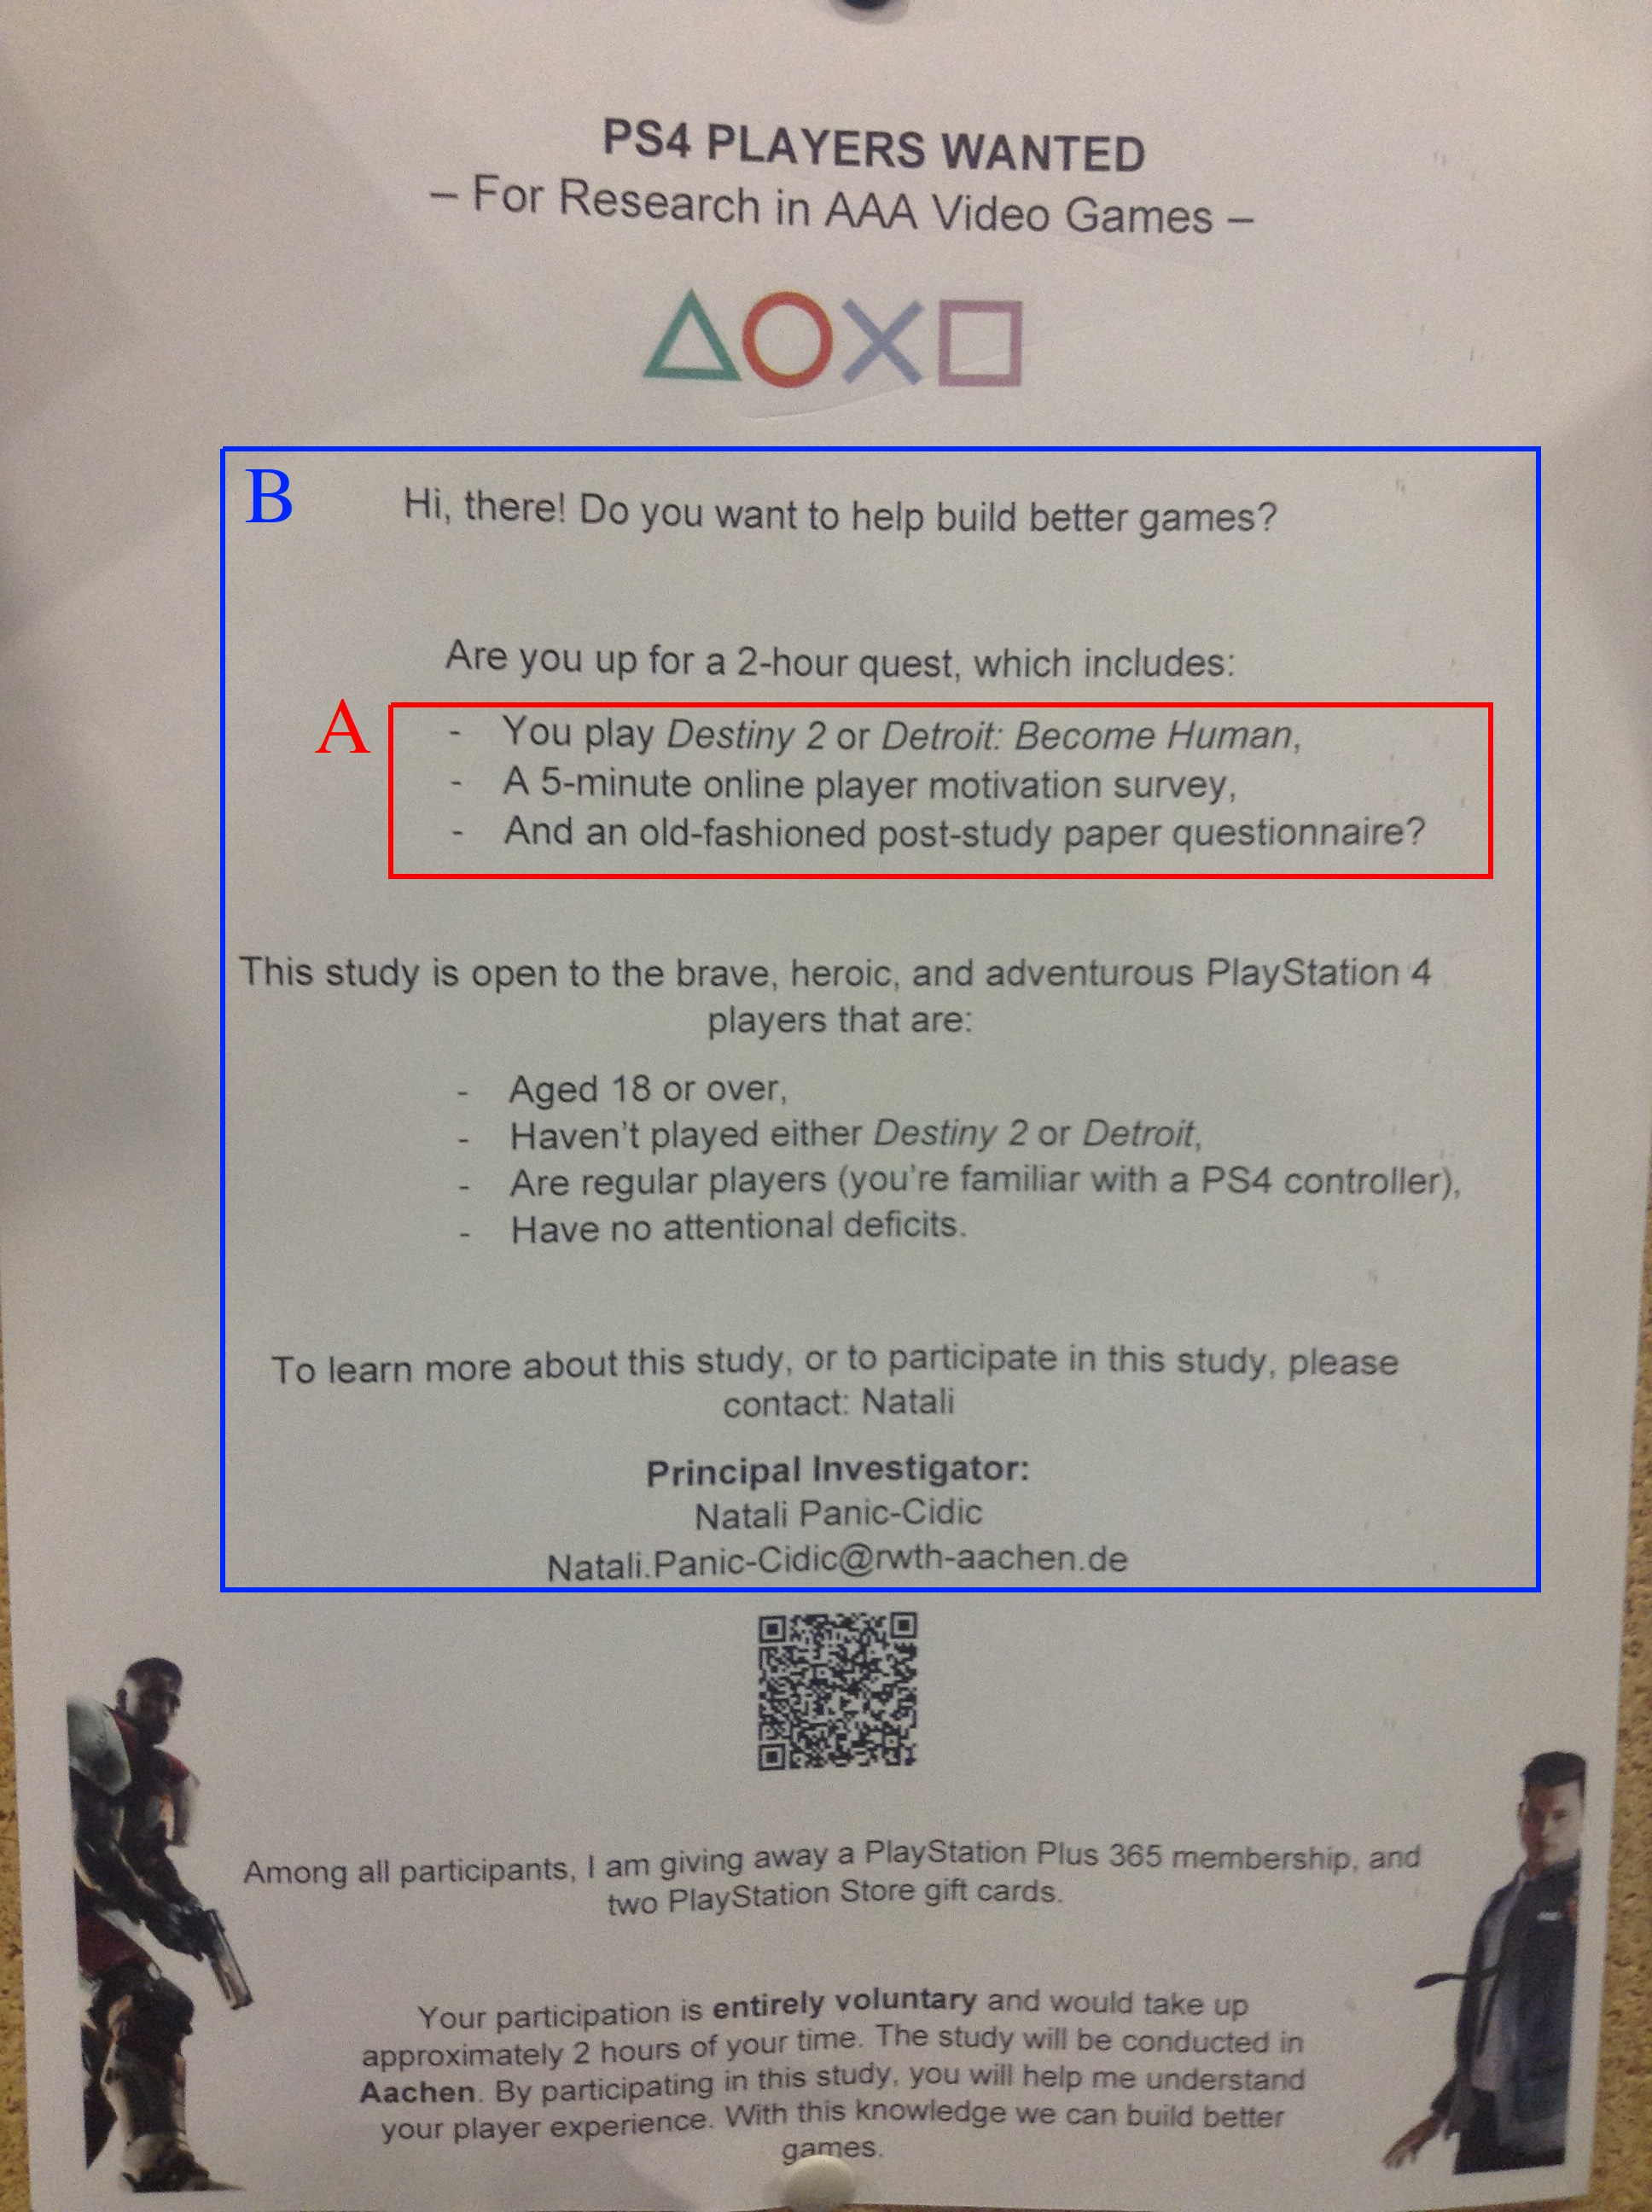
\includegraphics[clip, trim=0cm 0cm 0cm 0cm, scale=0.13]{./images/recruitment2.jpeg}
		\caption{PS4 Player Ad}
%		\label{fig:sub1}
	\end{subfigure}%
	\begin{subfigure}{.5\textwidth}
		\centering
%		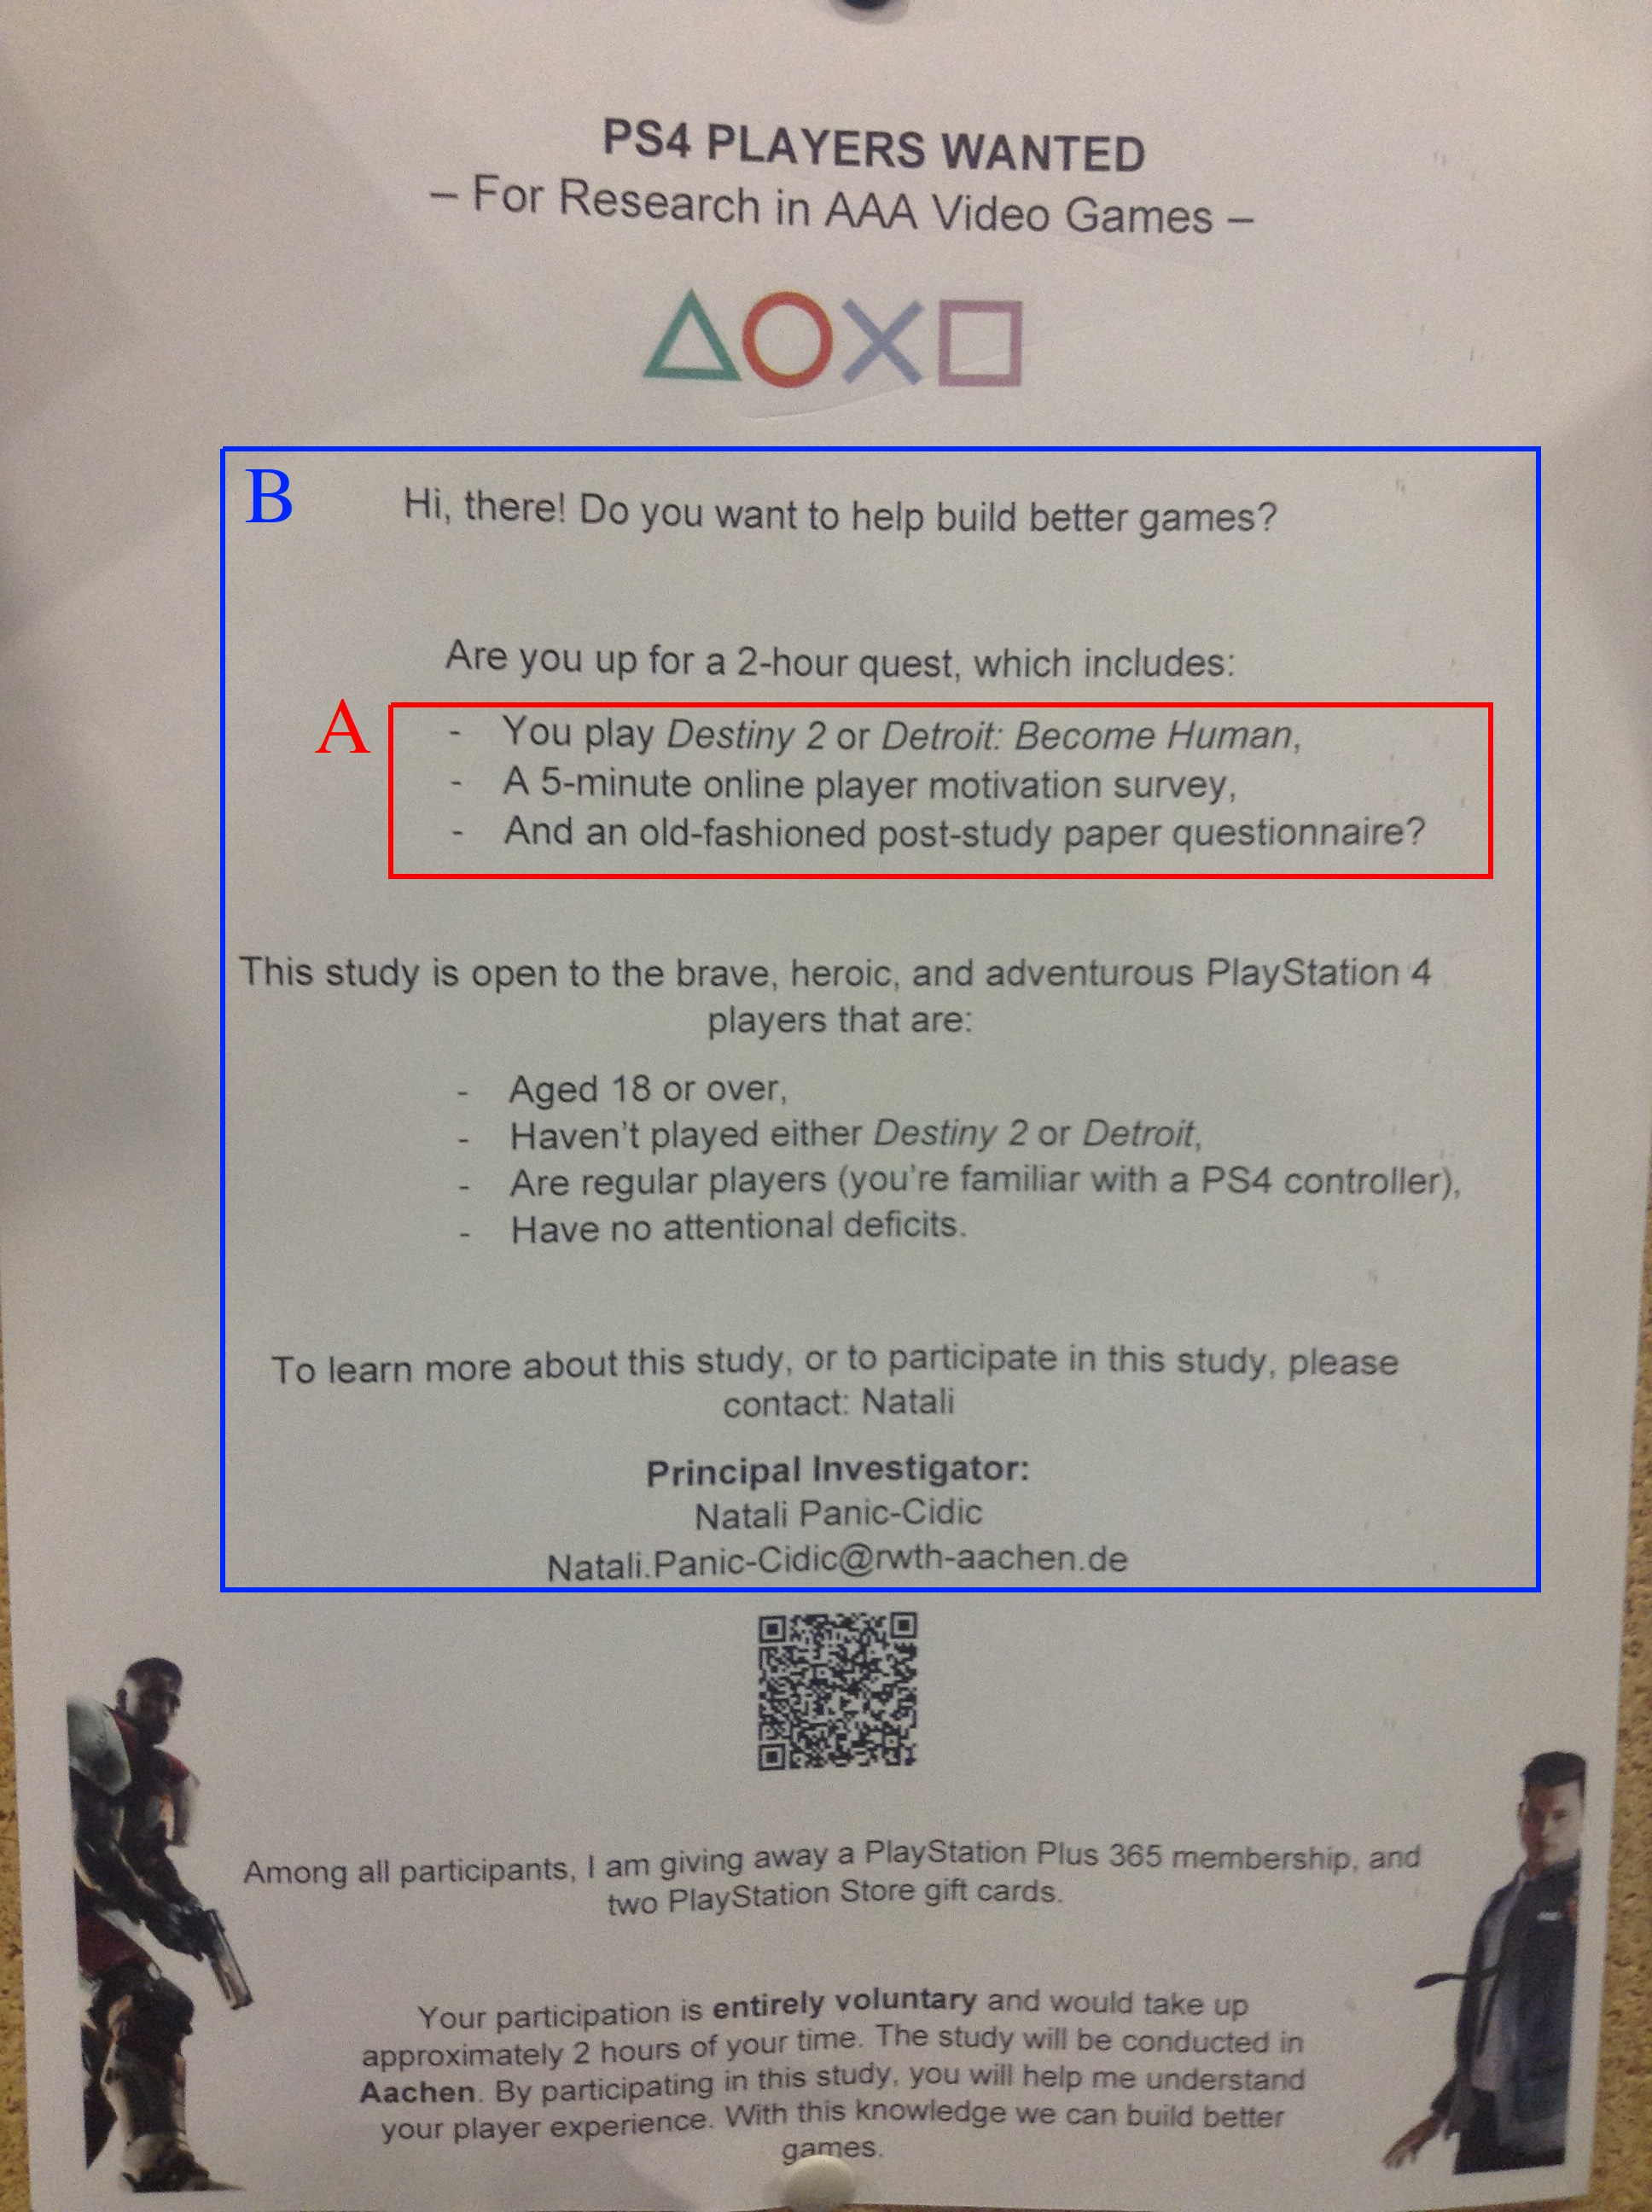
\includegraphics[clip, trim=0cm 0cm 0cm 0cm, scale=0.13]{./images/recruitment2.jpeg}
		\caption{add your image here with its short name, just change the path above and uncomment}
%		\label{fig:sub2}
	\end{subfigure}
%	\caption{Video Lan Client (VLC) Right-Click Menu}
	\label{fig:test}
\end{figure}

\begin{tabularx}{\textwidth}{|X|}
	\hline
		\textbf{Violations of Visual Design Principles}
		\\
	\hline
		\textbf{Violation \#1:} Contrast
		
		\\
		\textbf{Describe Violation:} Nearly no contrast, so many information with no distinction between nearly any text (titles have no contrast to the texts under them)
		
		
		\\
		\textbf{Why Bad?:} Makes it hard to distinguish between parts, and makes it hard to digest all the text. Assuming it has bold or larger subheaders (such as "Are you up for a 2-hour quest, which includes :" and "This study is open to brave, heroic, adventurous PS4 players that are:"), it would have been easier to understand the bill at the first glance. Although whitespace usage is not bad, he current form leads to more mental work distinguishing parts.
		
	\\
	\hline
	
		\textbf{Violation \#2:} Repetition
		
		\\
		\textbf{Describe Violation:} There is no consistent good repetition in the design. Aside from the same font size being used nearly everywhere, no part of the text and layout has been stepping forward to make a change in the view. This leads to dull-looking design. Note that there are tiny differences in the visual that steps forward like the main header "PS4 Players Wanted", and name of the investigator being bold, and two more; but those are few, thus, the style is repetitive in a negative sense, this repetitiveness does not help the user at all. 
		
		\\
		\textbf{Why Bad?:} User wants positive repetitiveness, and wants to know what to look at, how to continue reading text; in general, a good flow of style together with objects aligned well, like the CV example in the slides. In this, we have no such thing, the user is not 'guided' by the style that does not convey the idea of where to look. This is unstructured, or let's say repetitive in a bad manner that nothing gives out user any clue on what is important, where is the keypoints and so on.
		
	\\
	\hline	
	
		\textbf{Violation \#3:} Proximity
		
		\\
		\textbf{Describe Violation:} The list points(dashes) and the correspongding list items(texts) in the given bill have so much space in between them that them seem separate.
		
		\\
		\textbf{Why Bad?:} The list points and the list items observed as being separate does not help user digest them as coupled together, it is the other way, them seem separate. This leads to reading and observing difficulty, as they are not in their proximity, that is, not close enough.
		
		\\
		\hline	
		
	\textbf{Violation \#4:} 
	
	\\
	\textbf{Describe Violation:} 
	
	\\
	\textbf{Why Bad?:} 
	
	\\
	\hline	
	
	\textbf{Violation \#5:} 
	
	\\
	\textbf{Describe Violation:} 
	
	\\
	\textbf{Why Bad?:} 
	
	\\
	\hline	
	
	\textbf{Violation \#6:} 
	
	\\
	\textbf{Describe Violation:} 
	
	\\
	\textbf{Why Bad?:} 
	
	\\
	\hline	
	
	
	%	\raisebox{-\height}[0pt][0pt]{
\includegraphics[clip, trim=0cm 0cm 0cm 0cm, scale=0.2]{./images/redesign.png} }
	
	%	\hline
	
\end{tabularx}\\

%\begin{figure}[H]
%	\centering
%	\begin{subfigure}{.5\textwidth}
%		\centering
%		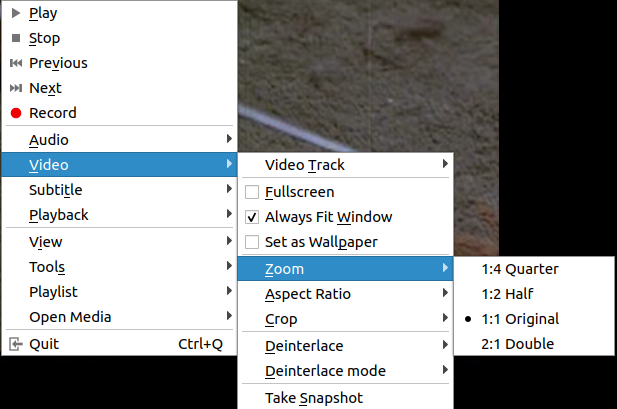
\includegraphics[clip, trim=0cm 0cm 0cm 0cm, scale=0.35]{./images/vlc_original.png}
%		\caption{Original}
%		\label{fig:sub1}
%	\end{subfigure}%
%	\begin{subfigure}{.5\textwidth}
%		\centering
%		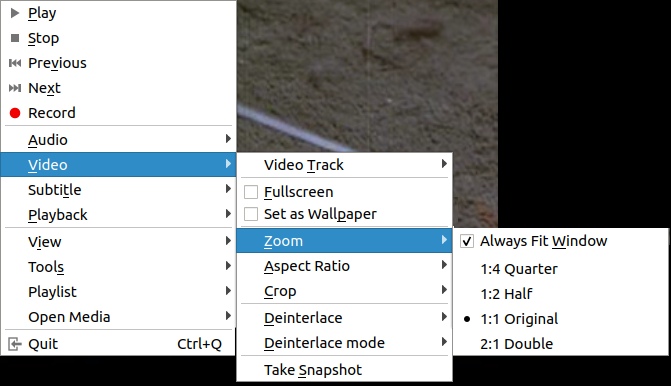
\includegraphics[clip, trim=0cm 0cm 0cm 0cm, scale=0.50]{./images/vlc_redesign.png}
%		\caption{Redesign}
%		\label{fig:sub2}
%	\end{subfigure}
%	\caption{Video Lan Client (VLC) Right-Click Menu}
%	\label{fig:test}
%\end{figure}

\end{document}}
